\documentclass[journal,twoside,web]{ieeecolor}
\usepackage{generic}
\usepackage{cite}
\usepackage{amsmath,amssymb,amsfonts}
\usepackage{algorithmic}
\usepackage{graphicx}
\usepackage{textcomp}
\usepackage{epstopdf}
\def\BibTeX{{\rm B\kern-.05em{\sc i\kern-.025em b}\kern-.08em
    T\kern-.1667em\lower.7ex\hbox{E}\kern-.125emX}}
\markboth{Miguel Faggioni}
{Author \MakeLowercase{\textit{et al.}}: Sistemas de Control Multivariable - Miguel Faggioni}
\begin{document}
	
\title{Control Óptimo - (Caso de estudio)}
\maketitle

\begin{abstract}
En el presente trabajo se estará analizando una planta asociada a la industria manufacturera con el fin de poner a pruebas este sistema a un esquema de control. En particular, se dará un enfoque optimo para estabilizar la planta de estudio. Por otro lado, se garantizara la robustez de la misma ante entradas tipo constantes.
\end{abstract}


\section{Descripción de la Planta}
En la producción de laminadoras de bandas en caliente, la calidad de las bandas es una de las más factores importantes para la satisfacción del consumidor. Por lo general se expresa en términos del espesor de la tira y el ancho de la misma. Dado que el proceso de laminación de bandas es parte del ultimo proceso que se debe completar para finalizar el producto es importante mantener altos niveles de calidad.

Es importante mantener una calidad de producción estable con un diseño de sistema de control en el proceso de laminación en caliente / frío. El proceso para ajustar el grosor de la tira esta principalmente controlado por un subsistema de válvulas, que a su vez controla un sistema de rodillos. Este proceso AGC esta modelado en general por la  ecuación del resorte

\begin{equation}
	h = S + \frac{P}{C}
\end{equation}

donde $C$ es la rigidez equivalente del soporte del molino, $h$ grosor de la lamina, $P$ la fuerza de rodadura y $S$ la brecha de los rodillos. La diferencia de espacio entre rodillos $\Delta S$es el parámetro clave a ser controlado por el sistema AGC, que conducirá a la cambio en la fuerza de rodadura $\Delta P$ basada en la ecuación del resorte. Esto da como resultado la fluctuación de los parámetros del rodillo horizontal de flexión y de deformación de corte, que a su vez causa desviaciones en la corona de la tira. Por otro lado en el sistema de control de la corona, el parámetro clave controlado es el cambio en las fuerzas de flexión $\Delta F$, que compensará de giro, pero puede conducir a la desviación de las fuerzas de los rodillos como una perturbación externa y luego causar un parámetro efecto de acoplamiento en el sistema AGC. Basado en lo anterior, el sistema de control de espesor de la corona se puede definir como un sistema multivariado típico con fuertes efectos de acoplamiento. Basado en investigaciones anteriores [2], [3] el sistema de control del grosor de la corona puede ser modelado por

\begin{equation}
	\begin{bmatrix}
		 \Delta h  \\
		 \Delta CR 
	\end{bmatrix} = G(s) \begin{bmatrix}
							 \Delta S  \\
							 \Delta F 
	  					\end{bmatrix}
\end{equation}


donde $\Delta CR$ es el cambio en el grosor de la corona y $\Delta h$ es el cambio en el espesor de la tira. Usando la teoría estándar de identificación de sistemas [4], el Parámetros del laminador de bandas en caliente para un punto de ajuste nominal. de 1700 mm y una velocidad de rodadura de 13 m/s puede ser determinada como [3]:

\begin{equation}
	\begin{bmatrix}
		 \Delta h  \\
		 \Delta CR 
	\end{bmatrix} = \begin{bmatrix}
			G_{11}(s) & G_{12}(s) \\
			G_{21}(s) & G_{22}(s)
	\end{bmatrix} \begin{bmatrix}
							 \Delta S  \\
							 \Delta F 
						\end{bmatrix}
\end{equation}

	\begin{equation}
		\begin{bmatrix}
		\Delta h  \\
		\Delta CR 
		\end{bmatrix} = \begin{bmatrix}
							\frac{0.00025s + 0.025}{0.00075s^2 + 0.065s + 1} & 	\frac{0.001}{0.0002s^2 + 0.03s + 1} \\
							\frac{0.00025s + 0.025}{0.00075s^2 + 0.065s + 1} & \frac{0.025}{0.0002s^2 + 0.03s + 1}
						\end{bmatrix} \begin{bmatrix}
											\Delta S  \\
											\Delta F 
										\end{bmatrix}
	\end{equation}

En la práctica, la velocidad de rodadura puede variar entre 10 y 16 m/s, Esto lleva al potencial de un cambio del 20\% en los parámetros. [2]. En términos generales, la incertidumbre puede ser cualquiera aditivo o multiplicativo. En el sistema de grosor de corona, La incertidumbre es multiplicativa, ya que se origina a partir de la velocidad de rodadura.


	\subsection{Modelo en Espacio de Estados}

Teniendo en cuenta que el sistema sera analizado por un sistema de control centralizado, debemos obtener el una realización en espacio de estados del caso de estudio. 
Para esto se uso las herramientas de conversión de sistemas SIMO que ofrece Matlab.

	\begin{equation}
		\begin{aligned}
			\begin{bmatrix}
				\dot{x_1}(t)  \\
				\dot{x_2}(t)  \\
				\dot{x_3}(t)  \\
				\dot{x_4}(t) 
			\end{bmatrix} = \begin{bmatrix}
								86.70 & -1333.30 & 0 & 0 \\
								1     & 0        & 0 & 0 \\
								0 & 0 & -150 & -5000 \\
								0 & 0 & 1 & 0 
							\end{bmatrix} \begin{bmatrix}
										x_1(t)  \\
										x_2(t)  \\
										x_3(t)  \\
										x_4(t) 
										\end{bmatrix} \\ + \begin{bmatrix}
												1 & 0 \\
												0 & 0 \\
												0 & 1 \\
												0 & 0
											\end{bmatrix}  + \begin{bmatrix}
																u_1(t) \\
																u_2(t)
															\end{bmatrix}
		\end{aligned}
	\end{equation}

	

\section{Análisis a Lazo Abierto del Sistema}

	\subsection{Estabilidad}
		
		Para este ítem se analizaran los auto-valores del sistema a lazo abierto teniendo en cuenta la representación en variables estados de la planta. De esta forma los mismos están localizados en la siguientes coordenadas del plano complejo
		
		\begin{equation}
			\begin{bmatrix}
				-66.67 \\
				-20.00 \\
				-100.00 \\
				-50.00
			\end{bmatrix}
		\end{equation}
		
		Los auto-valores están claramente localizados en el semi-plano izquierdo del plano complejo. Lo que permite concluir que el sistema es estable.		
		
	\subsection{Respuesta al Escalón}
	
	Teniendo en cuenta el modelo matemático del sistema, se realizara en análisis del mismo en lazo abierto, para esto se realizaron simulaciones haciendo uso 
	del paquete de Simulación Simulink.
	
	\begin{figure}[h]
		\begin{center}
			\includegraphics[width=7cm,height=4cm,keepaspectratio]{modelsimulink}
			\caption{Modelo de Simulación a Lazo Abierto\label{modelsimulink}}
		\end{center}
	\end{figure}
	
	Al someter a la planta a entradas constantes se obtuvieron los resultados que se aprecian en la Figura \ref{olstepresponse}.
	
	\begin{figure}[h]
		\begin{center}
			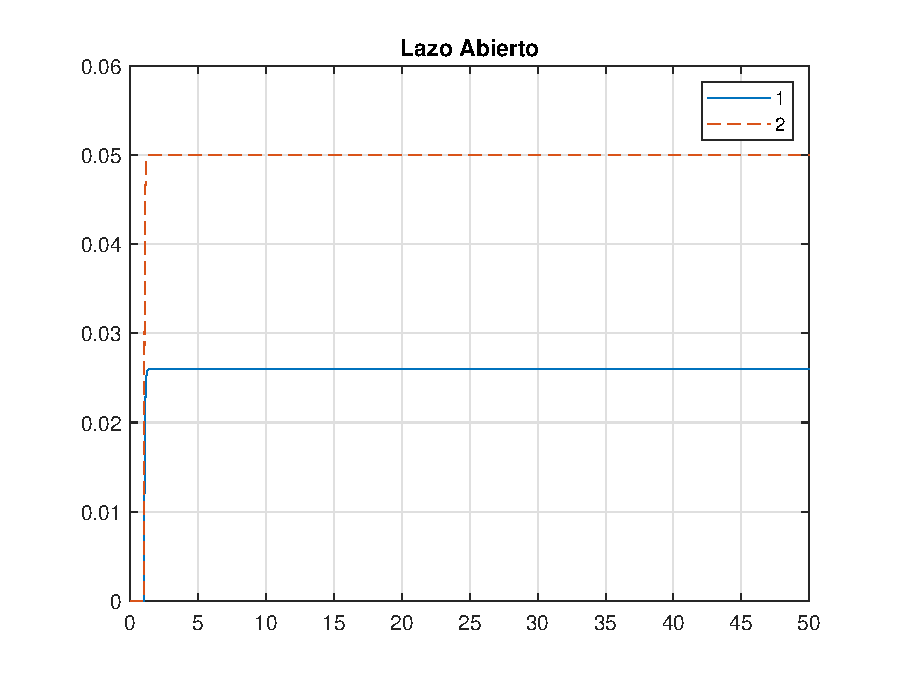
\includegraphics[width=6cm,height=6cm,keepaspectratio]{olstepresponse}
			\caption{ Respuesta del Sistema a lazo Abierto \label{olstepresponse}}	\end{center}
	\end{figure}		
	
	De la gráfica podemos observar que el sistema de forma natural es estable, sin embargo, posee un problema importante en estado estable, es notable error de estado estacionario.


\section{Control Optimo}

	Habiendo estudiado el sistema a lazo abierto de la planta de estudio, comencemos a establecer el esquema de control que permita dar solución al problema de regulación de forma optima, teniendo especial énfasis en proveer una respuesta robusta desde el punto de vista de perturbaciones a la planta. Para esto comencemos diseñando el observador del sistema.
	
		
	
	\subsection{Diseño de Observador}
	
	Como parte del sistema de control se diseño un observador Luenberger, cuyos autovalores están localizados en los siguientes puntos del plano complejo:
	
	\begin{equation}
		\lambda = \begin{bmatrix}
				-4 && -4 && -30 && -30
			\end{bmatrix}
	\end{equation}
	
	Haciendo uso de las herramientas de calculo disponibles podemos obtener que la matriz de ganancia del observador queda expresada en la siguiente ecuación:
	
	\begin{equation}
		L = \begin{bmatrix}
				279.177 && -11.167 \\
				-4.277 && 0.171 \\
				76.519 && 97.099 \\
				-0.833 && -0.895
			\end{bmatrix}
	\end{equation}
	
	A efectos de la simulación se estableció el siguiente diagrama de bloques.
	
	\begin{figure}[h]
		\begin{center}
			\includegraphics[width=8cm,height=8cm,keepaspectratio]{observer}
			\caption{ Diagrama de bloques del sistema observador \label{observer_system}}
		\end{center}
	\end{figure}
	
	\subsection{Diseño de Controlador}
	
	El diseño del controlador tomara en consideración una repuesta optima desde el punto de vista transitorio, adicionalmente se propondrá una respuesta robusta al ser capaz de rechazar perturbaciones. Para esto se propone el siguiente esquema de control.
	
	\begin{figure}[h]
		\begin{center}
			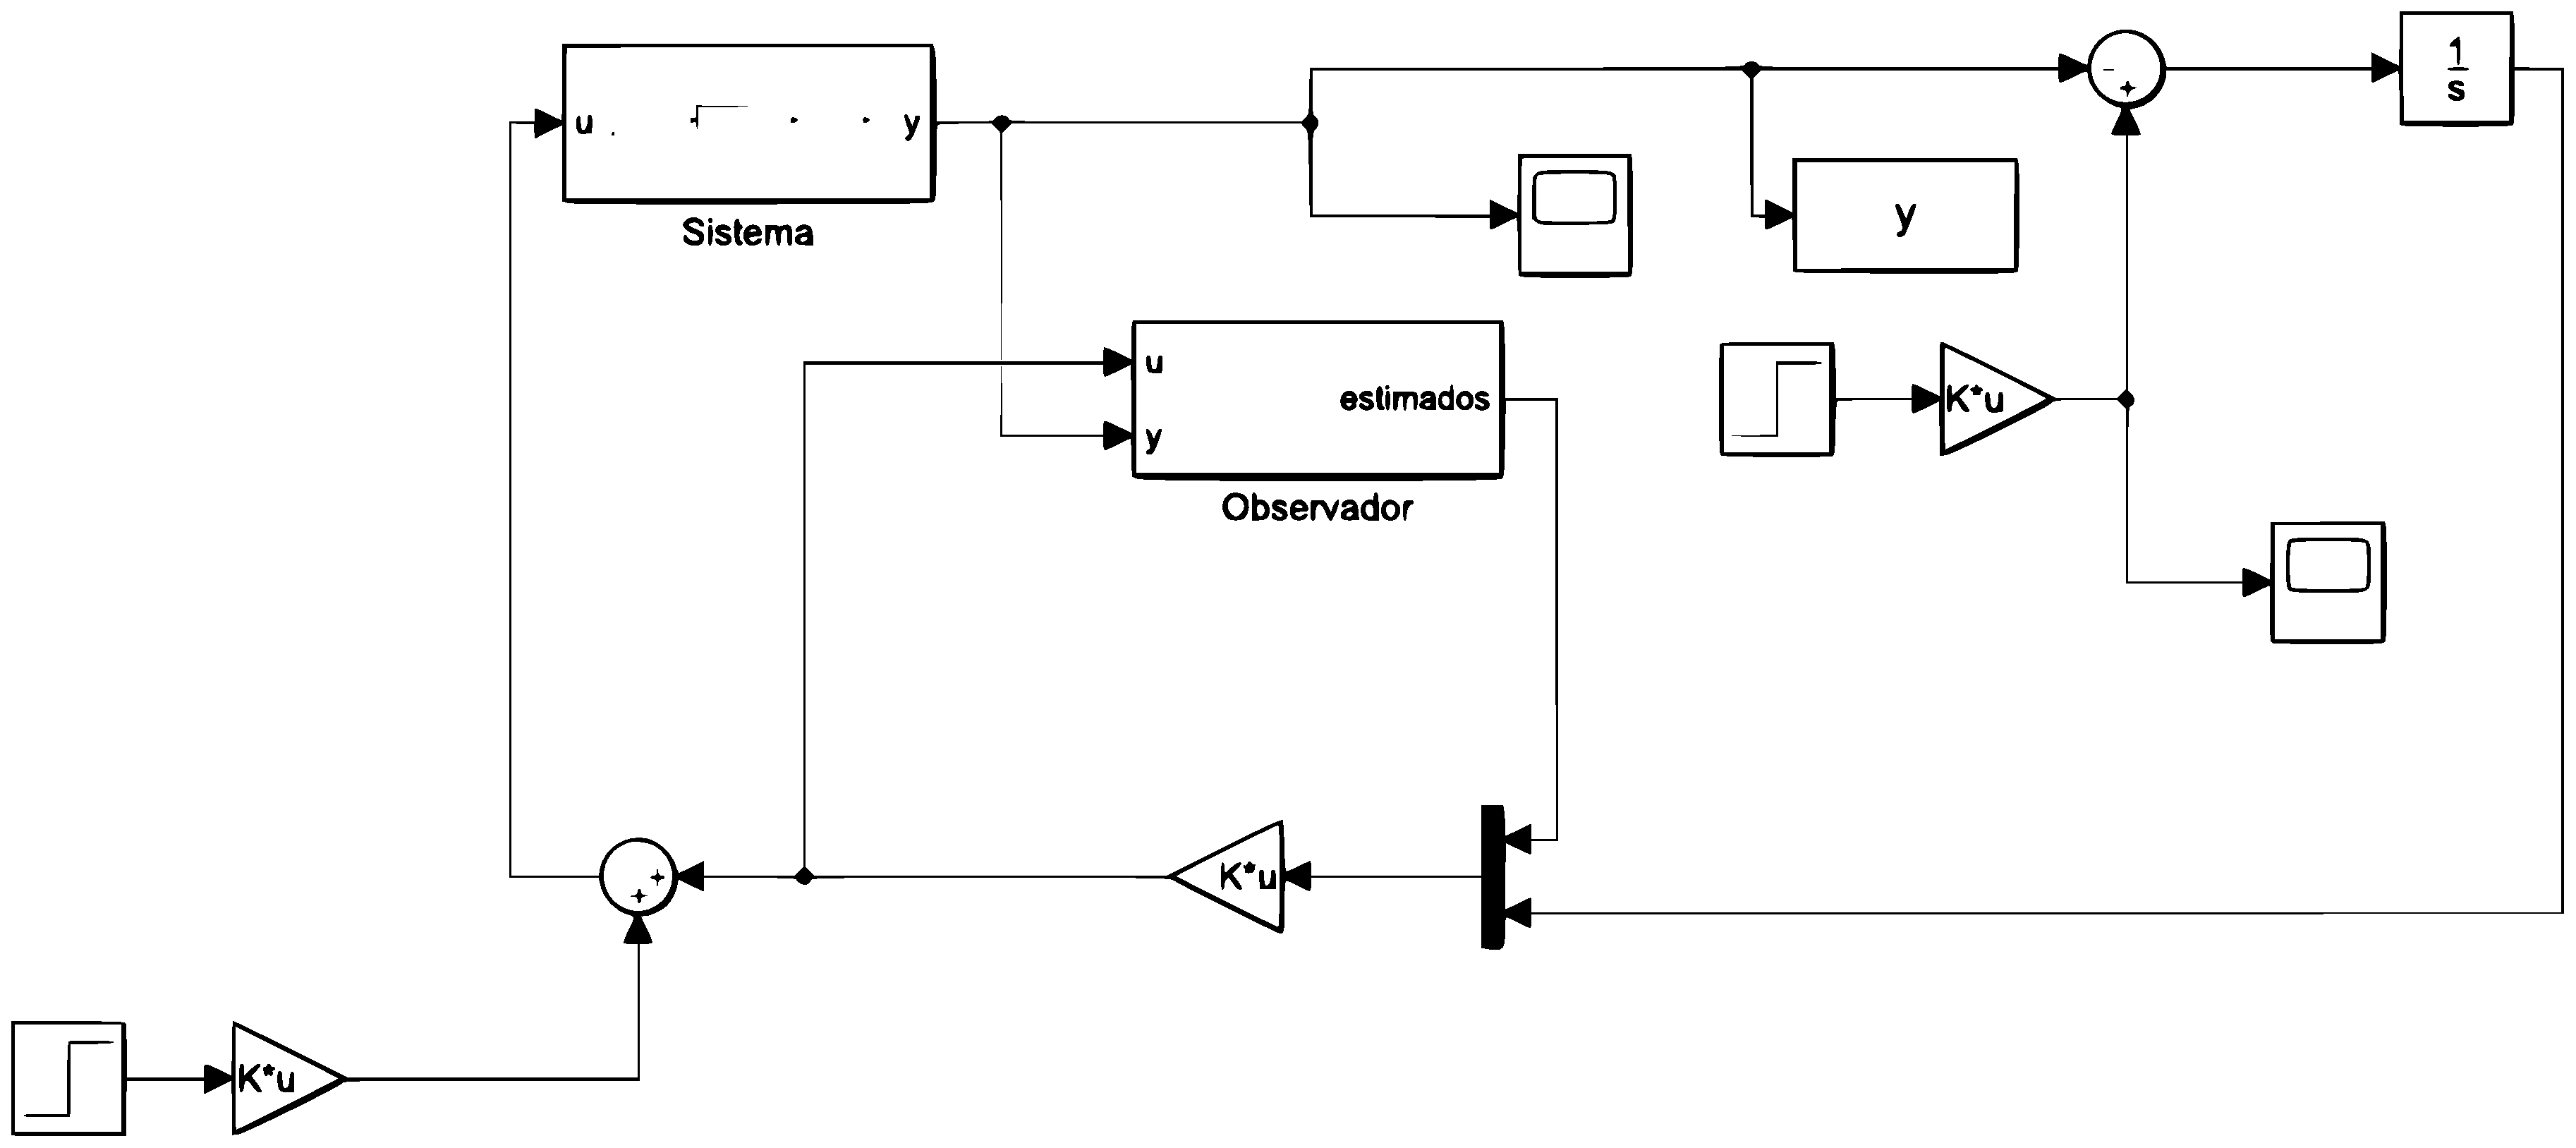
\includegraphics[width=8cm,height=8cm,keepaspectratio]{optimalcontrol}
			\caption{ Diagrama de bloques del sistema control \label{control-system}}
		\end{center}
	\end{figure}

	Vale la pena mencionar que el sistema fue modificado teniendo en cuenta el sistema aumentado, esto es, sistema e integrador. Así mismo se estableció el parámetro $\alpha$ en 0.90. Considerando esto, las matrices del estado aumentado quedan representadas en las siguientes ecuaciones. 
	
	\begin{equation}
	\resizebox{0.9\hsize}{!}{$%
		A^{'} = \begin{bmatrix}
					-85.8 & -1333.3 & 0 & 0 & 0 & 0 \\
					1     & 0.90 & 0 & 0 & 0 & 0 \\
					0     & 0 & -149.10 & -5000 & 0 & 0 \\
					0     & 0 & 1 & 0.90 & 0 & 0 \\
					-0.3  & -33.0 & 0 & -5 & -0.9 & 0 \\
					-0.3  & -3.3 & 0 & -125 & 0 & 0.9 \\
				\end{bmatrix}
				$%
			}%
	\end{equation}
	
	\begin{equation}
		B = \begin{bmatrix}
				1 & 0 \\
				0 & 0 \\
				0 & 1 \\
				0 & 0 \\
				0 & 0 \\
				0 & 0 
			\end{bmatrix}
	\end{equation}
	
	Se variaron de distintas formas las matrices de ponderación del modelo LQR, sin embargo no se logro obtener una repuesta muy favorable, por lo que se decidió trabajar con las matrices identidad de forma conveniente. Así pues, se pudo obtener una respuesta satisfactoria teniendo en cuenta los requerimientos establecidos. Esto se tradujo en una matriz de ganancia $K$, cuyos valores se muestran acontinuación.
	
	\begin{equation}
	\resizebox{0.8\hsize}{!}{$%
	K = \begin{bmatrix}
			1.81 & 132.91 & 0 & 0.007 & -72.31 & 2.89 \\
			0 & -21.69 & 1.81 & 270.1 & 7.23 & -72.30 \\		
		\end{bmatrix}
		$%
		}%
	\end{equation}
	
\section{Resultados}
	
	
	Luego de haber concluido la fase de experimentación y diseño se paso a simular el sistema tiendo en cuenta el diagrama de bloques de la figura \ref{control-system}. El mismo presenta la siguiente forma
	
	\begin{figure}[h]
		\begin{center}
			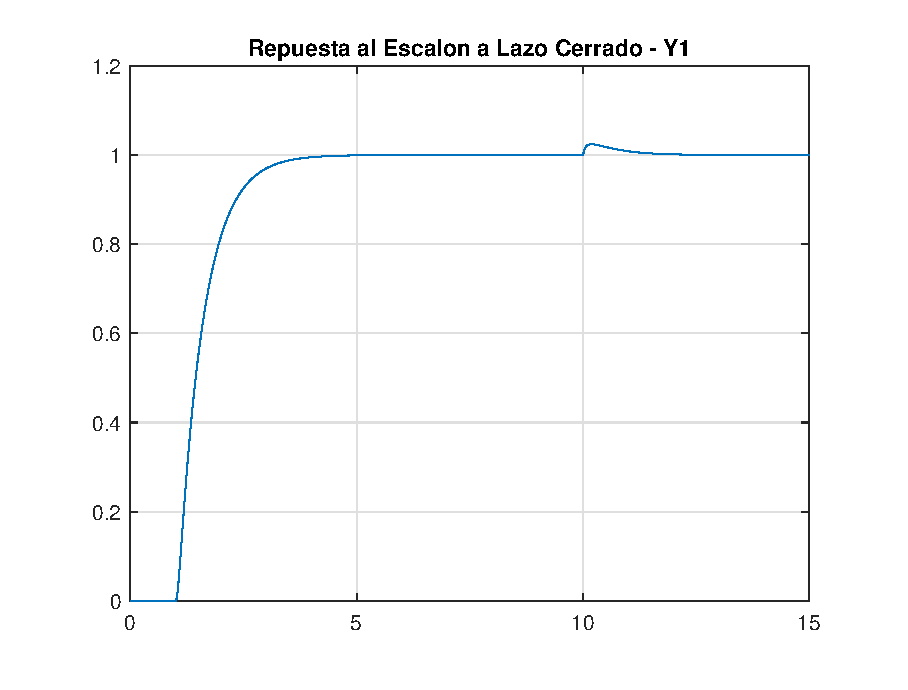
\includegraphics[width=8cm,height=8cm,keepaspectratio]{resp-cl-1}
			\caption{ Respuesta al escalon de la salida $y_1$ \label{control-system-cl-1}}
		\end{center}
	\end{figure}
	\begin{figure}[h]
		\begin{center}
			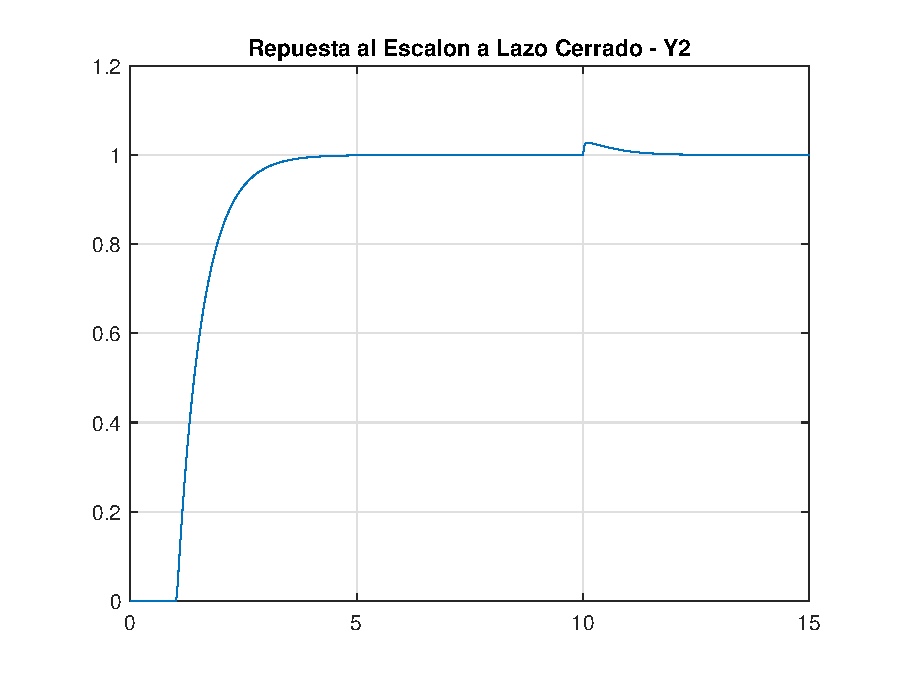
\includegraphics[width=8cm,height=8cm,keepaspectratio]{resp-cl-2}
			\caption{ Respuesta al escalon de la salida $y_2$ \label{control-system-cl-2}}
		\end{center}
	\end{figure}

	Como se puede apreciar en ambas gráficas, el sistema de control logra estabilizar la planta y mejorar la respuesta transitoria del sistema. Así mismo, se logra seguimiento en señales tipo constante. Mas aun, el seguimiento es robusto, ya que admite el rechazo a las perturbaciones de la misma naturaleza.
	
\section{Conclusión}

El siguiente caso de estudio permitió aplicar técnicas de control optimo a una planta de características reales. Así mismo, se logro un seguimiento robusto al aplicar el principio del modelo interno.


\begin{thebibliography}{00}
	\bibitem{b1} Kersting, S ``Direct and Inndirect Model Reference Adaptative Control for Multivariable Piecewise Affine Systems,'' IEEE Trans. Automat. Control, vol. 62, No. 11, pag 5634 - 5649 Nov. 2017.
	
	\bibitem{b2} Y. Sun,  ``The Model and Control of Cold and Hot Strip Mill,'' Beijing, China: Metallurgical Industry Press, 2010.
	
	\bibitem{b3} P. Jing, and C. Tonng,  ``Decoupling based robust control strategy for shape and gauge system,'' Inf. Control, vol. 40. no. 4, pp. 467-471, 2011.
	
	\bibitem{b4} Y. A. W. Shardt,  ``Statistics for Chemical and Proccess Engineers: A modern Approach,'' . Switzerland: Springer, 2015.

\end{thebibliography}

\end{document}


